\chapter{マルチスペクトル画像を用いた土の種類の識別}
\thispagestyle{empty}
\label{ch:SoilTypeDiscrimination}
\minitoc

\newpage
%%%%%%%%%%%%%%%%%%%%%%%%%%%%%%%%%%%%%%%%%%%%%%%%%%%%%%%%%%%%%%%%%%%%%%%%%%%%%%%
%==============================================================================
%はじめに
%==============================================================================
\section{はじめに}
本章では,非接触での走破性判定のために本研究で提案した,スペクトル画像を用いたコーン指数推定の最初のステップである,
スペクトル画像を用いた土の種類の識別の詳細について述べる.
本研究の提案手法において,本章で解説する部分を図\ref{fig:thesis_constitution_ch3}に茶色で示す.

% 本章では,スペクトル画像を用いて土の種類を識別する手法について述べる.
% 本研究では,土の種類を識別するため,スペクトル画像の中でも分光させる波長の数が多い
% ハイパースペクトル画像を使用する.

まず,\ref{sec:SoilTypeDiscriminationFromSpectrum}節において,
異なる土の種類がそれぞれ別の分光反射率スペクトルを持つことを利用して,
分光反射率スペクトルを用いて
土の種類の識別を非接触に行う手法について述べる.
% 分光反射率スペクトルを
% そして,分光反射率スペクトルを用いて土の種類を識別するためには,
% 詳細な分光反射率スペクトルの形状を知る必要性を述べる
なお,分光反射率スペクトルを用いて土の種類を識別するためには,
幅の狭い多数の波長帯の光の強さを記録する分光反射率スペクトルが
必要となるため,
波長分解能の高い分光反射率スペクトルを取得する必要があることを述べる.
% 波長幅の短い多数の波長帯から分光反射率を取得する必要があることを述べる.

次に,\ref{sec:ClassificationOfHyperspectralImage}節において,
土の種類を識別するための波長分解能の高い分光反射率スペクトルを取得するため,
スペクトル画像のなかでも分光させる波長帯の数が非常に多いマルチスペクトル画像を用いることを述べる.
% ハイパースペクトル画像を用いた土の種類の識別について述べる.

最後に,\ref{sec:PreliminaryExperimentOfDiscrimination}節において,
\ref{sec:SoilTypeDiscriminationFromSpectrum}節と\ref{sec:ClassificationOfHyperspectralImage}節で解説した手法の
有効性を確認するために行った,マルチスペクトル画像を用いて土の種類を識別する検証実験について述べる.

\begin{figure}[p]
	\begin{center}
	\centering
	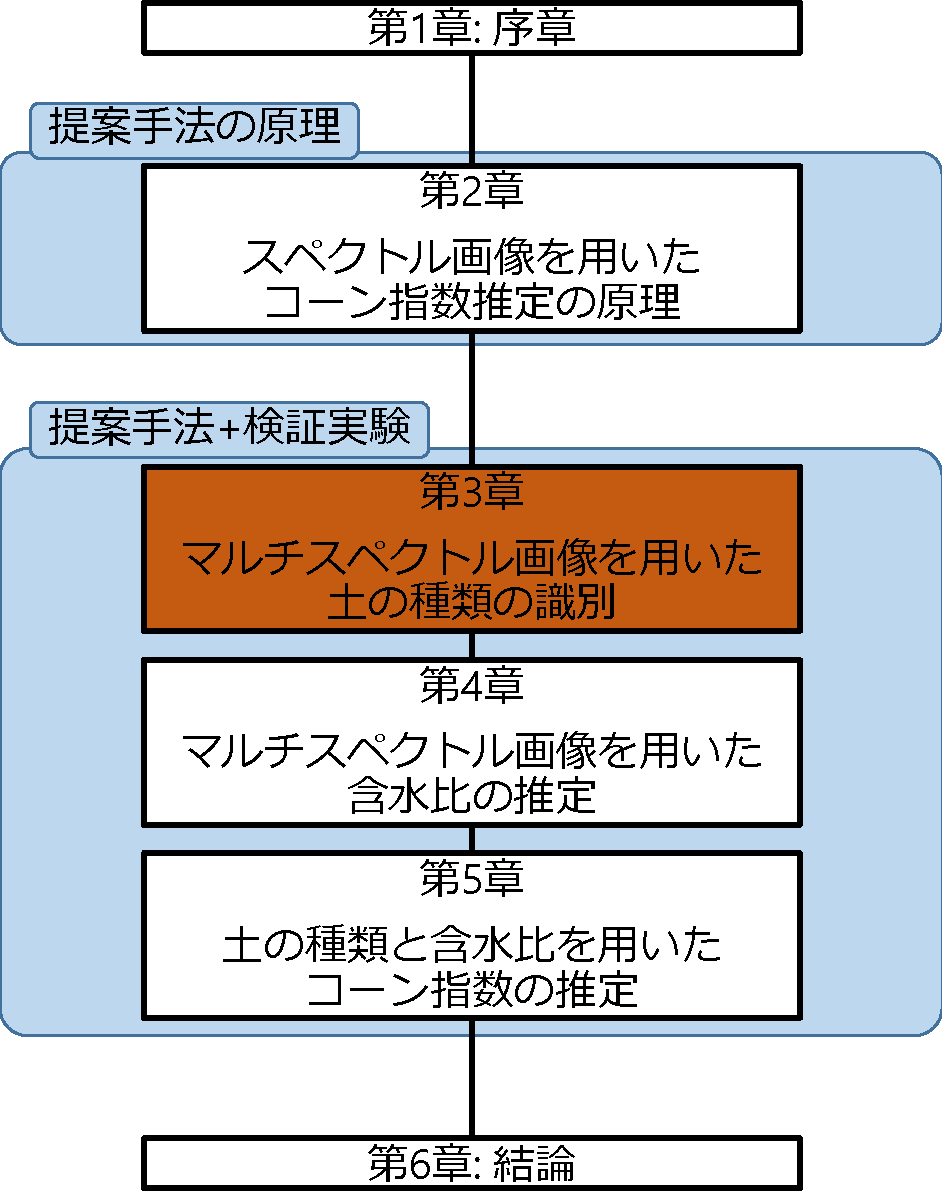
\includegraphics[width=8cm]{./Ch3_SoilTypeDiscrimination/Fig/thesis_constitution_ch3_compressed.pdf}
	\caption{本章で解説する部分(茶色の部分)}\label{fig:thesis_constitution_ch3}
	\end{center}
\end{figure}


\clearpage


%==============================================================================
%分光反射率スペクトルを用いた土の種類の識別
%==============================================================================
\section{分光反射率スペクトルを用いた土の種類の識別}
\label{sec:SoilTypeDiscriminationFromSpectrum}

\ref{sec:PrimciplesOfConeindexEstimation}節で述べた通り,
土の基本的な性質を示す土質パラメータはコーン指数に大きく影響する.
そこで,本研究では,
様々な土のうち,
% コーン指数に大きく影響する,土の基本的な性質を示す
土の基本的な性質を示す土質パラメータの中でも
外部の状況に左右されない,土に固有の土質パラメータである,土の粒子の鉱物組成,有機物含有量,粒度分布,球形率が同じ土を
同じ種類の土と定義した.
従って,土の種類が異なると,これらの外部の状況に左右されない土に固有の土質パラメータも異なることになる.

また,\ref{sec:SpectrumAndMaterialRelationship}節で述べた通り,
物質は,その分子や原子の構造,または物質を構成する微粒子の大きさや形,表面の凹凸によって,
光の波長ごとの反射,散乱,吸収,そして放射の度合いが異なるため,
物質の種類と状態が異なると分光反射率スペクトルも異なる.
従って,土の種類が異なると土の粒子の材質や直径の分布,形,表面の粗さも異なるため,
土の種類ごとに異なる分光反射率スペクトルを持つ.
本研究ではこれを利用して,
予め土の種類ごとに測定した分光反射率スペクトル
を用いて土の種類を識別する.

土の種類ごとに異なる分光反射率スペクトルを持つ例を図\ref{fig:spectrum_for_different_soiltype}に示す.
図\ref{fig:spectrum_for_different_soiltype}に示したグラフにおいて,縦軸は分光反射率,横軸は波長を示す.
また,グラフ中の黒,赤,青の3本の曲線は,それぞれ異なる土の種類である,粘性土,火山灰質粘性土,礫質土の分光反射率スペクトルを示す.
この3種類の土の種類は,異なる場所で採取された異なる種類の土である.
このうち,粘性土と火山灰質粘性土は,共に,0.075mm未満の,粘土と呼ばれる土の粒子が最も大きな割合を占める土である.
一方,礫質土は,2mmから75mmまでの,礫と呼ばれる土の粒子が最も大きな割合を占める土である.% 引用
上記の3種類の土の画像を図\ref{fig:different_soiltype_image}に示す.

\begin{figure}[p]
	\begin{center}
		\begin{tabular}{c}

			\begin{minipage}[t]{\linewidth}
			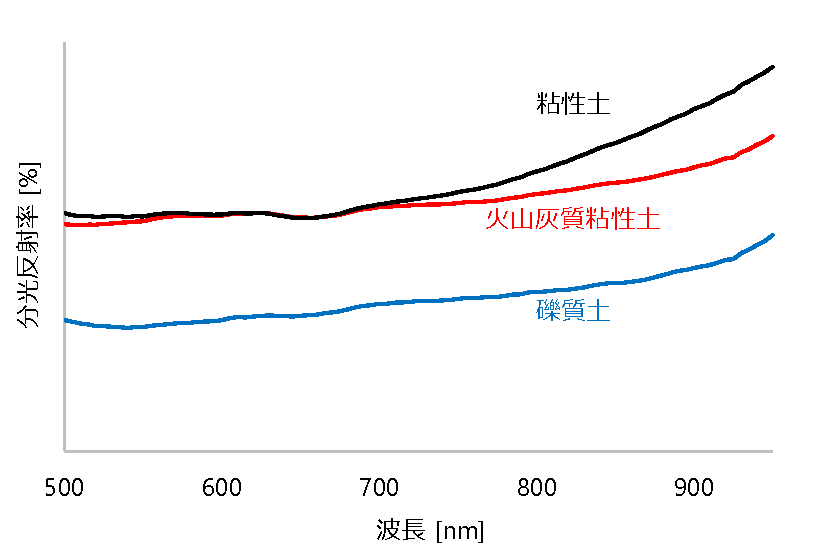
\includegraphics[width=13cm]{./Ch3_SoilTypeDiscrimination/Fig/spectrum_for_different_soiltype_compressed.pdf}
			\caption{土の種類ごとに異なる分光反射率スペクトル}\label{fig:spectrum_for_different_soiltype}
			\vspace{2cm}
			\end{minipage}

			\\

			\begin{minipage}[t]{0.33\linewidth}
			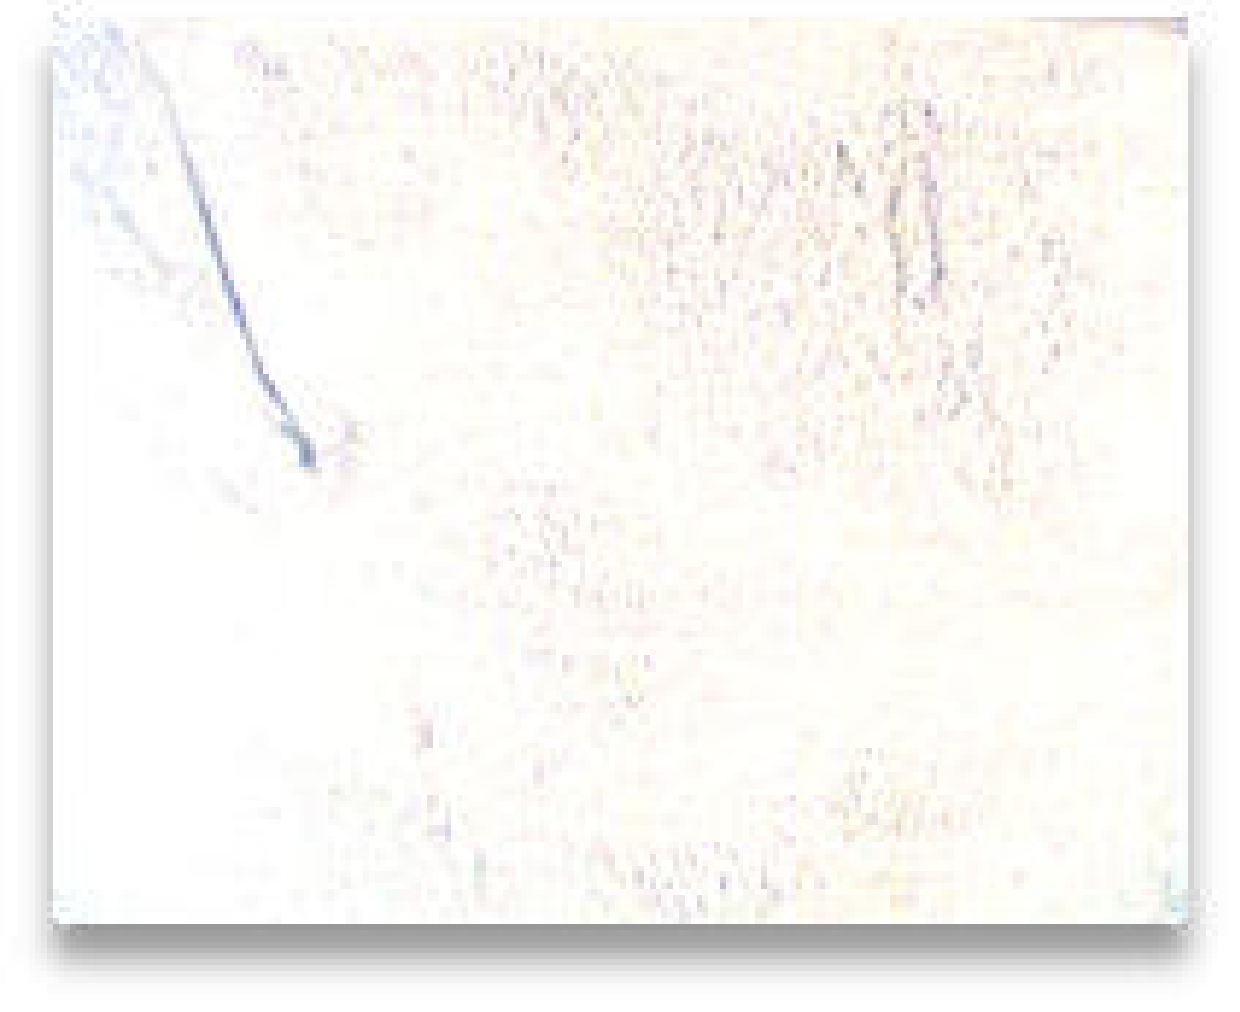
\includegraphics[width=4cm]{./Ch3_SoilTypeDiscrimination/Fig/A_Fu_image_compressed.pdf}
			\caption*{粘性土}
			\end{minipage}

			\hfill

			\begin{minipage}[t]{0.33\linewidth}
			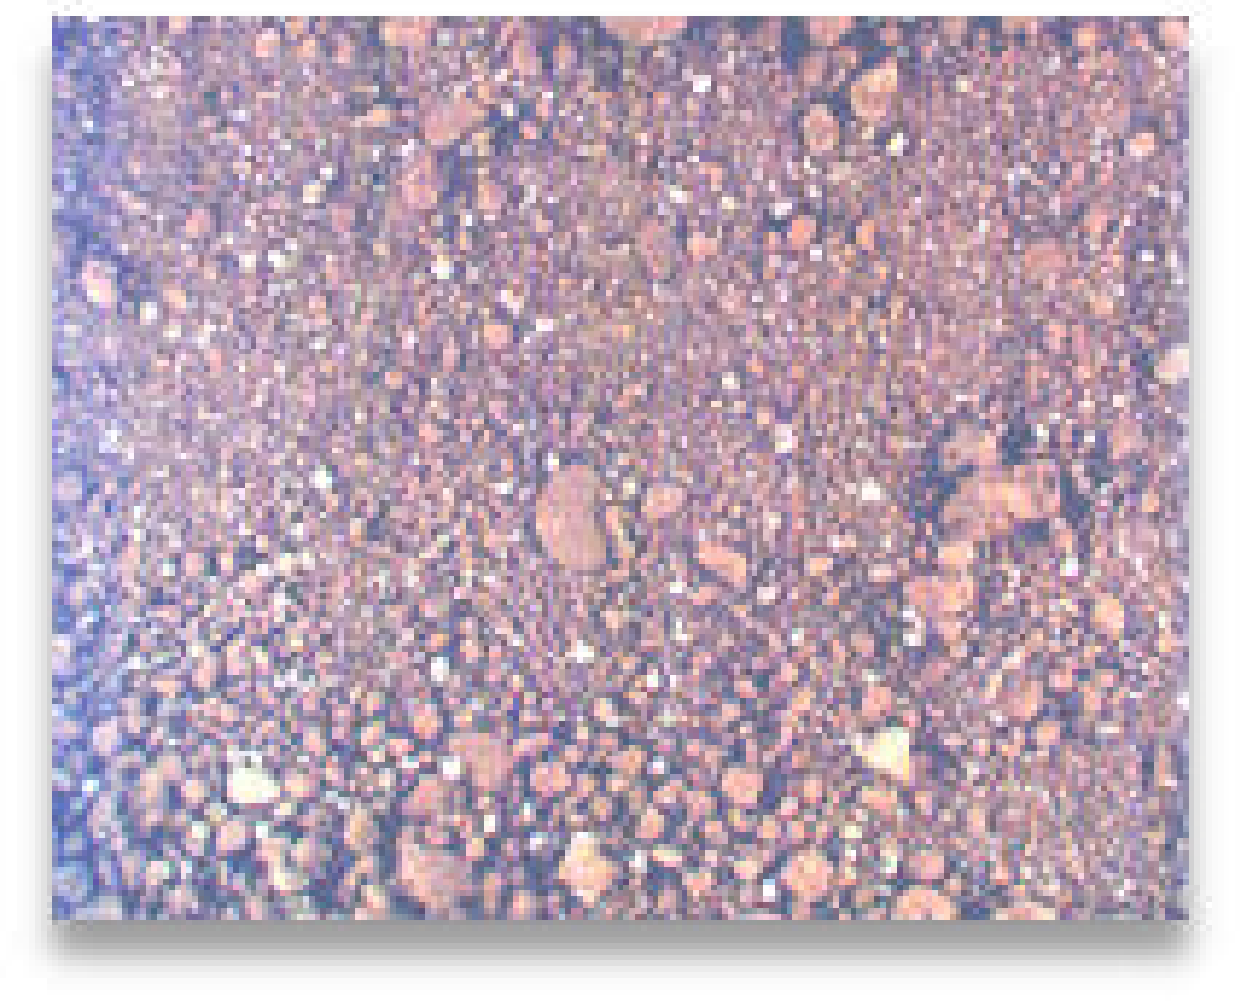
\includegraphics[width=4cm]{./Ch3_SoilTypeDiscrimination/Fig/B_Is_image_compressed.pdf}
			\caption*{火山灰質粘性土}
			\end{minipage}

			\hfill

			\begin{minipage}[t]{0.33\linewidth}
			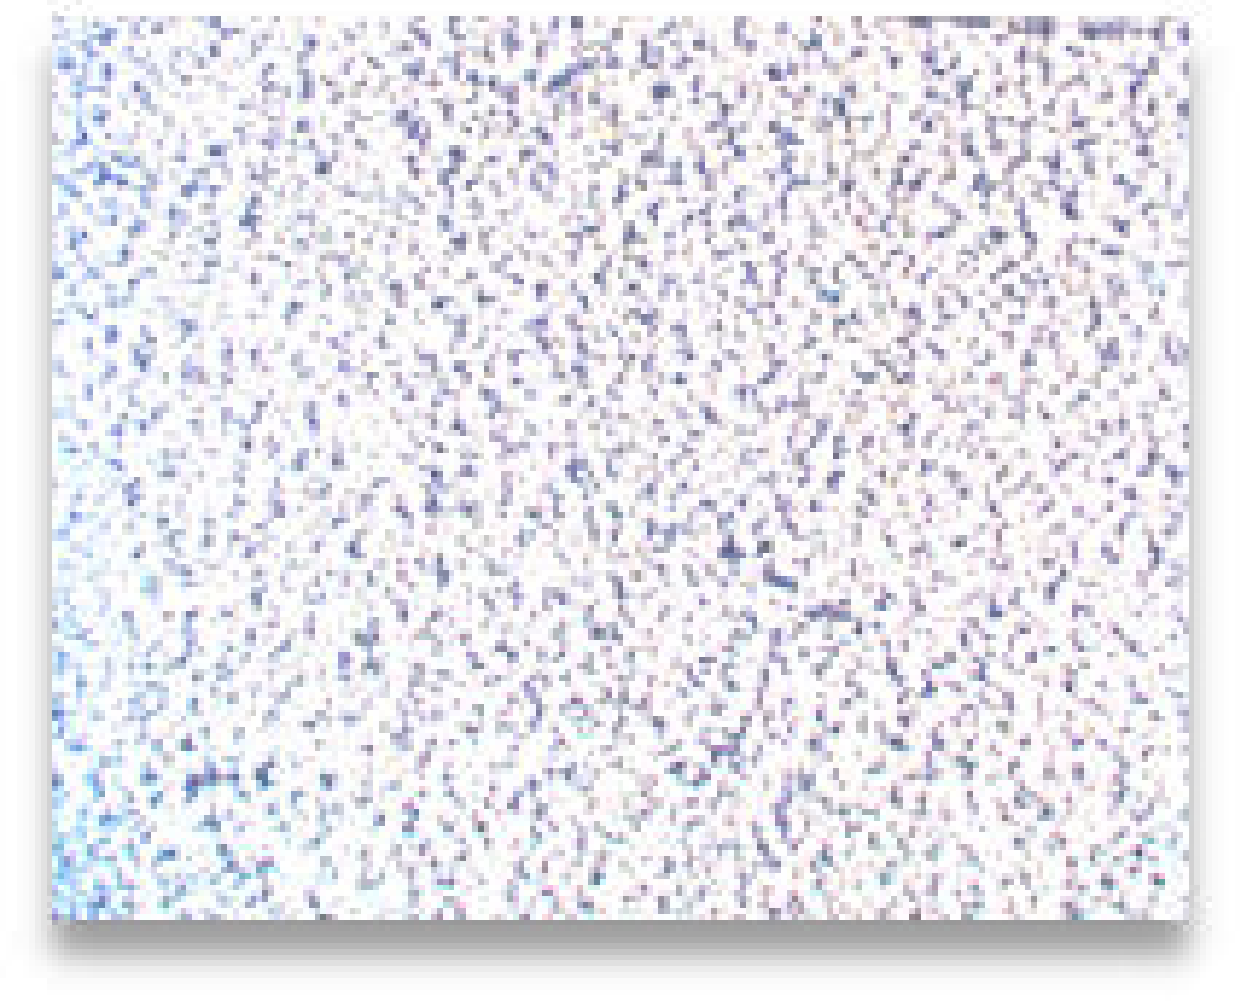
\includegraphics[width=4cm]{./Ch3_SoilTypeDiscrimination/Fig/C_K1_image_compressed.pdf}
			\caption*{礫質土}
			\end{minipage}

		\end{tabular}
		\caption{分光反射率スペクトルを比較した3種類の異なる土の画像}\label{fig:different_soiltype_image}
	\end{center}
\end{figure}

\clearpage

図\ref{fig:spectrum_for_different_soiltype}より,
土の種類ごとに異なる分光反射率スペクトルが存在することが分かる.
% ここにもう1つ項(土の種類の識別に必要な分光反射率スペクトルの要件)を入れて,波長分解能についてより詳しく述べる
% なぜ高い波長分解能が必要なのか
% 1つの節に1つの項だけでは不自然
しかし,多くの種類の土を分光反射率スペクトルで識別するためには,
図\ref{fig:spectrum_for_different_soiltype}に示したような,非常に多くの波長帯の光の強さを記録する
% 波長分解能の高い why
分光反射率スペクトル
を知る必要がある.
6種類の土を本研究と同様の手法で,取得する波長帯の数が異なる画像から識別した際の識別精度を図\ref{fig:discrimination_accuracy_by_wavelength_number}に示す.図\ref{fig:discrimination_accuracy_by_wavelength_number}において,縦軸は土の種類の識別精度,
横軸は各画像で取得する波長帯の数を示す.
図\ref{fig:discrimination_accuracy_by_wavelength_number}より,
波長帯の数が多くなる程,画像を用いた土の種類の識別精度が向上することが分かる.

非常に多くの波長帯の光の強さを記録する
分光反射率スペクトルを取得するためには,入射光を幅の短い多数の波長帯に分光させる,
波長分解能の高いスペクトル画像を用いる必要がある.
そのために,本研究では,スペクトル画像の中でも,波長分解能の高い
マルチスペクトル画像を使用する.
この波長分解能の高いマルチスペクトル画像を用いて,非常に多くの波長帯の光の強さを記録する分光反射率スペクトル
を取得し,土の種類の識別に利用する.

\begin{figure}[b]
	\begin{center}
	\centering
	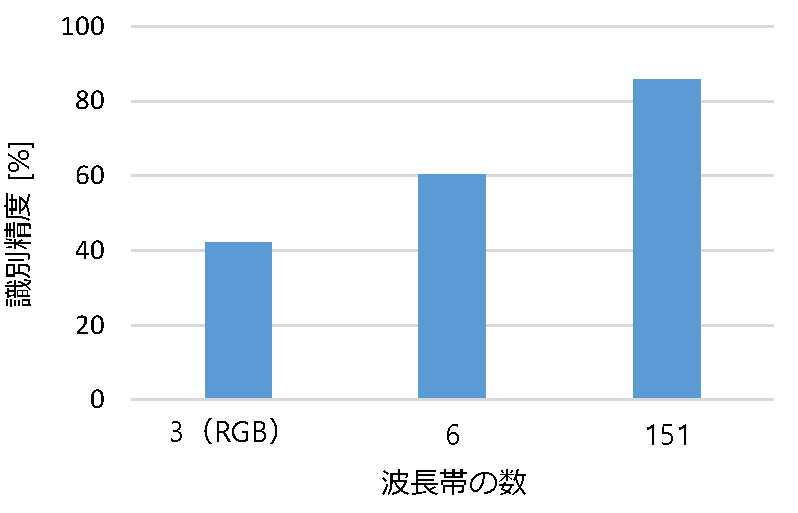
\includegraphics[width=10cm]{./Ch3_SoilTypeDiscrimination/Fig/discrimination_accuracy_by_wavelength_number_compressed.pdf}
	\caption{取得する波長帯の数が異なる画像を用いた土の種類の識別精度の比較}\label{fig:discrimination_accuracy_by_wavelength_number}
	\vspace{1cm}
	\end{center}
\end{figure}

\clearpage


\section{マルチスペクトル画像の分類}
\label{sec:ClassificationOfHyperspectralImage}

\subsection{波長帯の数が非常に多いマルチスペクトル画像}
\label{ssec:HyperspectralImage}

マルチスペクトル画像とは,
スペクトル画像の中でも,一般的なRGB画像が取得するR,G,Bの3波長帯以外の波長帯も取得するマルチスペクトル画像というスペクトル画像を用いる\cite{中野1996}.

本研究において土の種類の識別に用いるマルチスペクトル画像は,
対象とする物体を走査するように撮影するため,
マルチスペクトル画像を構成する画素ごと,あるいは画素の列ごとに% "ピクセル"にすると目立つので,"画素"で統一
入射光を分光させて得た分光反射率スペクトルを記録し,
それを終えると,次の画素や画素の列の
入射光を分光して分光反射率スペクトルを記録し始める.
そのため,
画素ごとに,撮影時にその画素内に映し出された物質の分光反射率スペクトルが記録されている.
従って,マルチスペクトル画像から分光反射率スペクトルを取得するには,
画素ごとに取得する.

また,\ref{sec:HyperAndMultiImages}節で述べた,本研究でも使用するような,
入射光を分光して記録する波長帯の数が非常に多いマルチスペクトル画像は
1980年代に衛星に搭載されるようになり,
広範囲に渡る地表の鉱物資源の分布の調査,植生の分布の調査,生態系の監視などに使用されている\cite{Underwood2003}\cite{Kruse2003}\cite{Ustin2004}\cite{Haboudane2004}\cite{Clark2005}.

\clearpage

\subsection{ニューラルネットワークによる分類}
\label{ssec:NeuralNetWork}

\ref{ssec:HyperspectralImage}項において述べた通り,
本研究では,マルチスペクトル画像から取得した分光反射率スペクトルを用いて土の種類を識別する.
分光反射率スペクトルは非線形であり,また他の物質からの光の散乱によって本来の形状を乱されることも多いので,
ニューラルネットワークを用いて識別を行う.
分光反射率スペクトルを用いて土の種類を識別するために,
分光反射率スペクトルを示すベクトルを入力層とし,出力層のノードの数を識別する土の種類の数,
中間層を入力層の約半分の数のノードで構成した,3層のニューラルネットワークを用いる.
まず,マルチスペクトル画像から画素ごとに記録されている分光反射率スペクトルを取得し,
取得した分光反射率スペクトルがホワイトアウトまたはブラックアウトしていないかどうかを確認して,
ニューラルネットワークに入力する.
なお,ホワイトアウトもブラックアウトもしていない分光反射率スペクトルの数が100以下のマルチスペクトル画像は
土の種類の識別には使用しないこととする.
ホワイトアウトもブラックアウトもしていない分光反射率スペクトルの数が100より多いマルチスペクトル画像から
取得した分光反射率スペクトルに土の種類のラベルを付け,土の種類の識別を行う.
分光反射率スペクトルはマルチスペクトル画像が取得する波長帯の数の成分を持つベクトルとして存在し,
それぞれの成分は0以上1未満となる.
分光反射率スペクトルを示す,マルチスペクトル画像が取得する波長帯の数の成分を持つベクトルを,
そのままニューラルネットワークの入力層として使用する.
本研究で使用するニューラルネットワークは,3層の全結合層から構成されている.
上記で解説した入力層と全結合する中間層は,入力層の約半分の数のノードで構成されており,
活性化関数にはReLUを使用する.
中間層と全結合する出力層は,識別する土の種類の数と同じ数のノードで構成されており,
活性化関数にはSoftmaxを使用する.
中間層と出力層の間ではドロップアウトを行い,ドロップアウトする割合は0.2に設定する.
このニューラルネットワークの最適化にはRMSporpを使用し,学習率は0.001に設定する.

マルチスペクトル画像から画素ごとに記録されている分光反射率スペクトルを取得し,
ニューラルネットワークを用いて土の種類を識別する様子を,
図\ref{fig:neuralnetwork}に示す.
図\ref{fig:neuralnetwork}において,
左側にあるのがマルチスペクトル画像であり,
右側にあるのが本研究で使用したニューラルネットワークである.
また,マルチスペクトル画像の上にある赤いひし形は1つの画素を示しており,
各画素ごとに記録された分光反射率スペクトルを取得して,
それをニューラルネットワークに入力する様子を示している.

図\ref{fig:neuralnetwork}に示すニューラルネットワークにおいて,
本研究では入力層のノードの数$C_r$が151,中間層のノードの数$m$が65となる.
また,出力層のノードの数$n$は,この後の\ref{sec:PreliminaryExperimentOfDiscrimination}節で述べる
マルチスペクトル画像から土の種類を識別する検証実験ではその検証実験で識別する土の種類の数である10となり,
\ref{sec:ConeindexEstimationExperiment}節で述べる,
コーン指数の推定の検証実験ではその検証実験で識別する土の種類の数である6となる.

\begin{figure}[b]
	\begin{center}
	\centering
	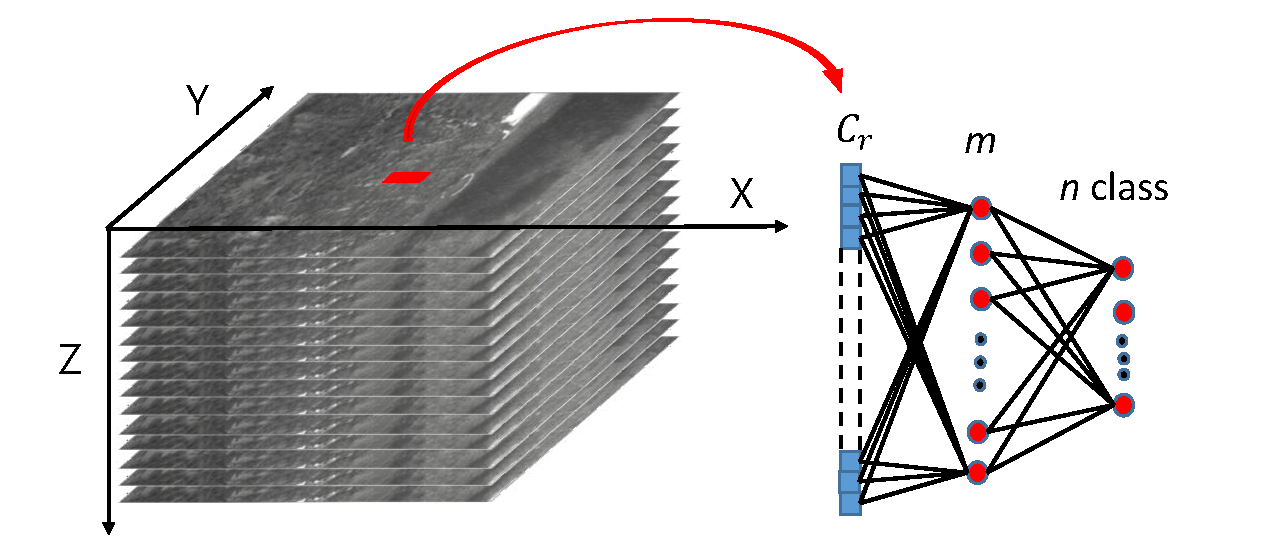
\includegraphics[width=13cm]{./Ch3_SoilTypeDiscrimination/Fig/neuralnetwork_for_hyperspectralimage_compressed.pdf}
	\caption{マルチスペクトル画像を分類するニューラルネットワーク}\label{fig:neuralnetwork}
	\vspace{6cm}
	\end{center}
\end{figure}

\clearpage

%==============================================================================
%土の種類を識別する検証実験
%==============================================================================
\section{土の種類を識別する検証実験}
\label{sec:PreliminaryExperimentOfDiscrimination}

\ref{sec:SoilTypeDiscriminationFromSpectrum}節と\ref{sec:ClassificationOfHyperspectralImage}節で
解説した,マルチスペクトル画像から取得した分光反射率スペクトルを用いた土の種類の識別の有効性を確認するため,
検証実験を行った.
% また,本研究において土の種類の識別に使用するマルチスペクトル画像は,入射光を分光して記録する波長帯の数が非常に多いため,
% \ref{sec:HyperAndMultiImages}節で述べたように,\ref{sec:PreliminaryExperimentOfDiscrimination}節で使用する,
% 取得する波長帯の数が非常に多いマルチスペクトル画像のことをハイパースペクトル画像と呼称する.

\subsection{実験環境}
\label{ssec:DiscriminationExperimentSetting}

今回の検証実験の目的は,
土の種類の違いによる分光反射率スペクトルの違いから,土の種類の識別を行うことができるか確認することである.
そのため,土の種類の違い以外の要因による分光反射率スペクトルの変動をなるべく除外する必要がある.
本研究の目的は,災害現場における建設機械の非接触での走破性判定である.
従って,マルチスペクトル画像の撮影時には屋外で太陽光を光源とする.
しかし,太陽光は時間や天候などの条件によって光量が変動するため,
屋外で同じ物質をマルチスペクトル画像で撮影しても,撮影時の環境の条件によって
取得した分光反射率スペクトルが変動する可能性がある.
% 従って,今回の検証実験において,太陽光を光源として使用することは困難である.
そこで,太陽光に似たスペクトルを持っているハロゲンランプを光源としてマルチスペクトル画像を
撮影することにした.
これにより,環境の条件の変化による土の分光反射率スペクトルの変動を除外しつつ,
太陽光を光源とした場合と似た分光反射率スペクトルをマルチスペクトル画像から取得することができる.
今回の検証実験におけるマルチスペクトル画像の撮影時の撮影機材の配置を図\ref{fig:discrimination_experiment_setting}に示す.% 実験の概要は"様子",各種の数値で表現できる場合は"条件"とする
図\ref{fig:discrimination_experiment_setting}に示す通り,土を入れた容器を中心にして,周囲を囲むように3つのハロゲンランプを配置して,
マルチスペクトル画像の撮影に十分な光量を確保した.
そして,マルチスペクトル画像を撮影するためのマルチスペクトルカメラを,土を入れた容器の直上に配置して撮影を行った.
なお,今回の検証実験で使用したマルチスペクトルカメラは,エバ・ジャパン株式会社製のNH-7である.
NH-7の写真と具体的な仕様を,それぞれ図\ref{fig:hyperspectral_camera}と表\ref{tbl:hyperspectral_camera}に示す.
% また,NH-7の具体的な仕様を表\ref{tbl:hyperspectral_camera}に示す.
また,土の含水比を0$\%$に揃えて撮影を行った.

\begin{figure}[p]
	\begin{center}
		\begin{tabular}{c}

			\begin{minipage}[t]{\linewidth}
			\hspace{3cm}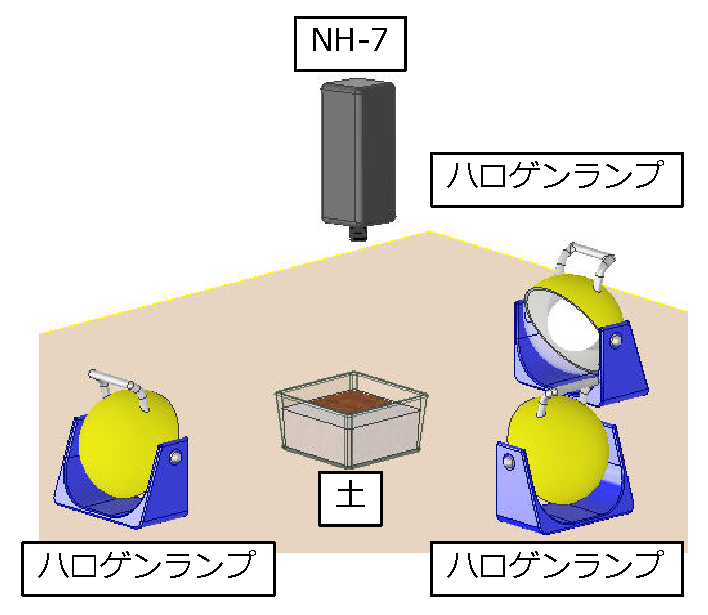
\includegraphics[width=7cm]{./Ch3_SoilTypeDiscrimination/Fig/discrimination_experiment_setting_compressed.pdf}
			\caption{検証実験における撮影機材の配置}\label{fig:discrimination_experiment_setting}
			\vspace{2cm}
			\end{minipage}

		\end{tabular}
	\end{center}
\end{figure}

\begin{figure}[b]
	\begin{center}
		\begin{tabular}{c}

			\begin{minipage}[b]{0.5\linewidth}
			% \vspace{1.5cm}
			% \hspace{4cm}
			\hspace{1cm}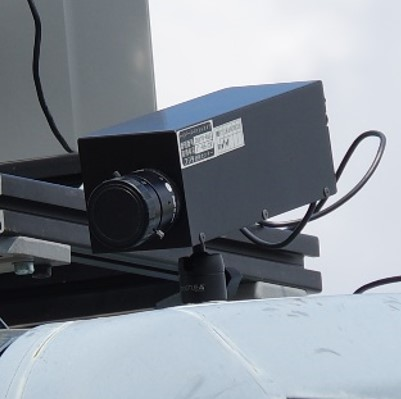
\includegraphics[width=5cm]{./Ch3_SoilTypeDiscrimination/Fig/hyperspectral_camera.jpg}
			\caption{NH-7}\label{fig:hyperspectral_camera}
			\vspace{1.5cm}
			\end{minipage}

			\hfill

			\begin{minipage}[b]{0.5\linewidth}
			\vspace{-2cm} % 表の高さを右のマルチスペクトルカメラの仕様を示した表と合わせる
			\tblcaption{NH-7の仕様}\label{tbl:hyperspectral_camera}
			
				\begin{center}
					% \hspace{4cm}
					\begin{tabular}{|c|c|} \hline
					製品名 & NH-7 \\ 
					(メーカー)& (エバジャパン)\\ \hline
					波長 & 350 $\sim$ 1100nm \\ 
					   &(ピッチ: 5nm)\\ \hline
					波長帯数 & 151 \\ \hline
					\end{tabular}
				\end{center}
			% \vspace{0.2cm} % 図表のタイトルを右と合わせる
			\vspace{3cm}
			\end{minipage}

		\end{tabular}
	\end{center}
\end{figure}

\clearpage

\subsection{実験データ}
\label{ssec:DiscriminationExperimentalProcedure}

今回の検証実験では,全国の異なる場所から集めた10種類の土を使用した.
集めた10種類の土のうち,5種類は,土を構成する土粒子のうち半分以上の直径が0.075mm以上75mm未満の粗粒土,
残りの5種類が,土を構成する土粒子のうち半分以上の直径が0.075mm未満の細粒土である.
また,5種類の細粒土は,さらにその土の起源によって,粘性土と火山灰質粘性土に分けられる.
今回使用した10種類の土のRGB画像を図\ref{fig:discrimination_experiment_data}に示す.
図\ref{fig:discrimination_experiment_data}のRGB画像の下には
,それぞれの土が粗粒土,粘性土,火山灰質粘性土のどれであるかを記載した.
また,この10種類を,表にある通り,以降AからJの名前で呼称する.

\begin{figure}[p]
	\begin{center}
		\begin{tabular}{c}

			\begin{minipage}[t]{0.33\linewidth}
			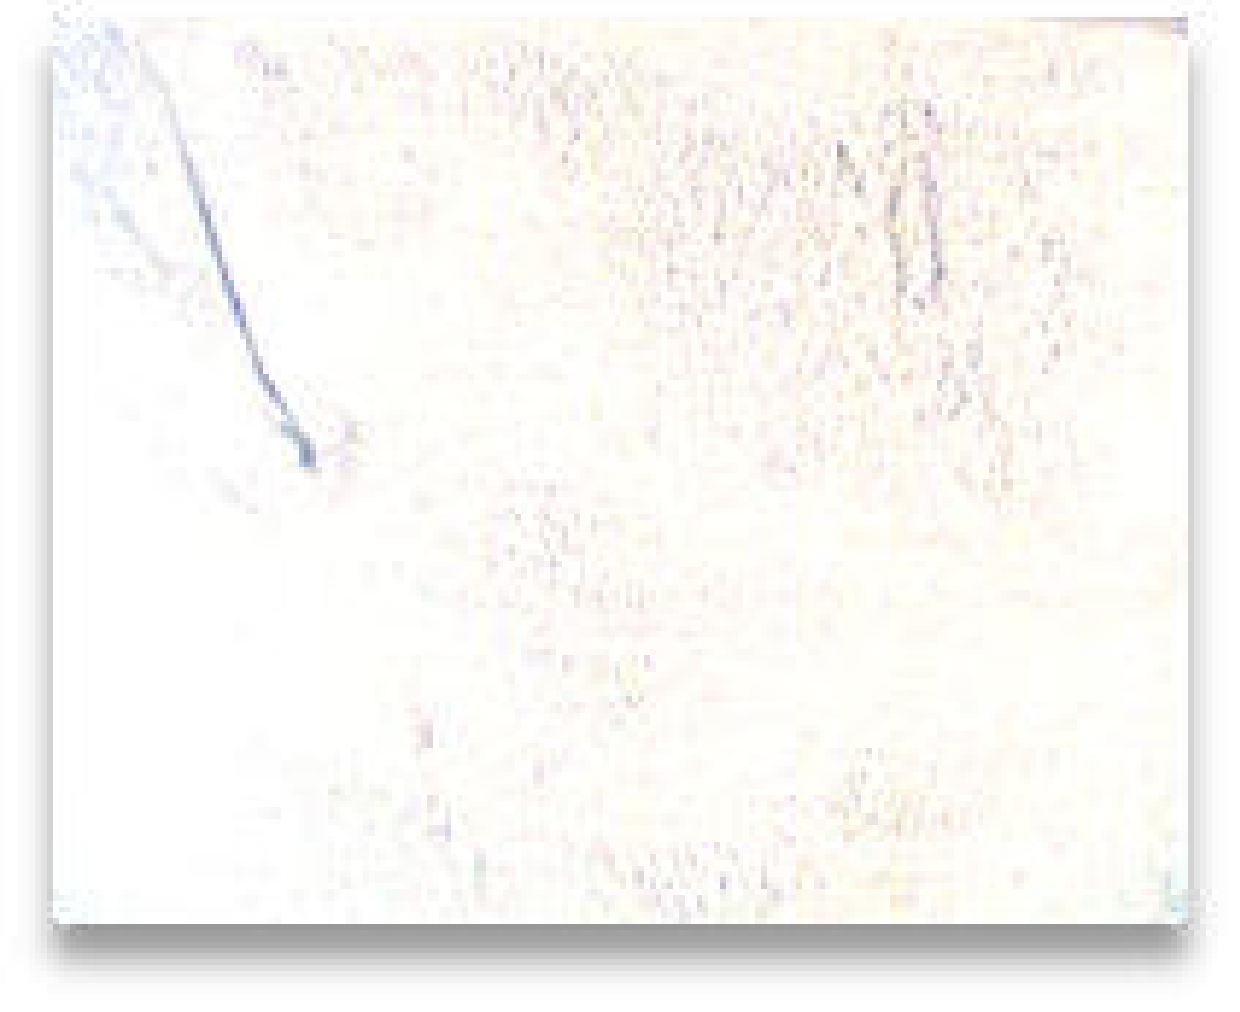
\includegraphics[width=4cm]{./Ch3_SoilTypeDiscrimination/Fig/A_Fu_image_compressed.pdf}
			\caption*{(a)土の種類A(粘性土)} % 京都府
			% \vspace{2cm}
			\end{minipage}

			\begin{minipage}[t]{0.33\linewidth}
			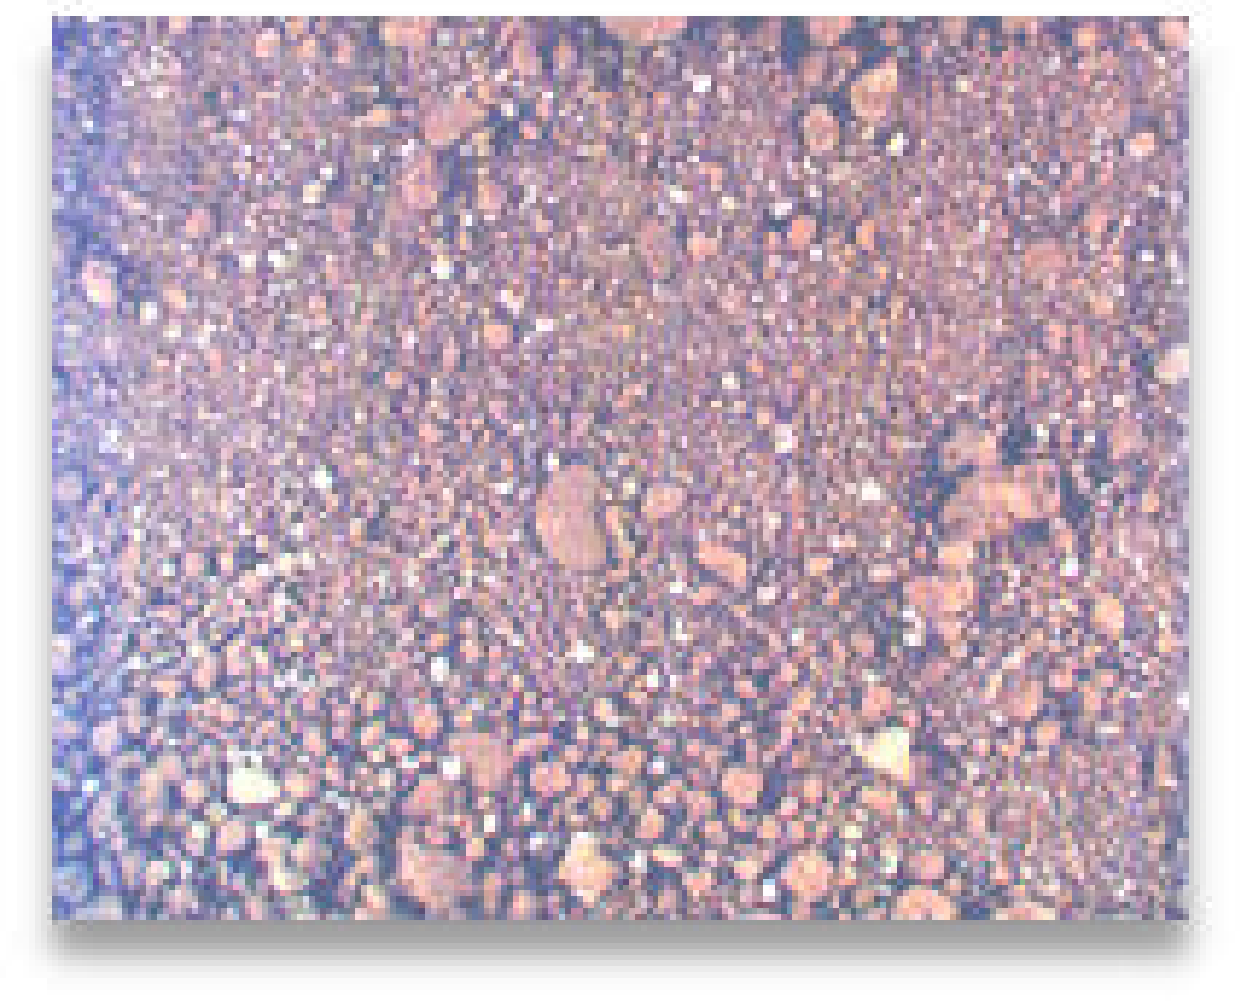
\includegraphics[width=4cm]{./Ch3_SoilTypeDiscrimination/Fig/B_Is_image_compressed.pdf}
			\caption*{(b)土の種類B(火山灰質粘性土)} % 神奈川県伊勢原市
			\end{minipage}

			\hfill

			\begin{minipage}[t]{0.33\linewidth}
			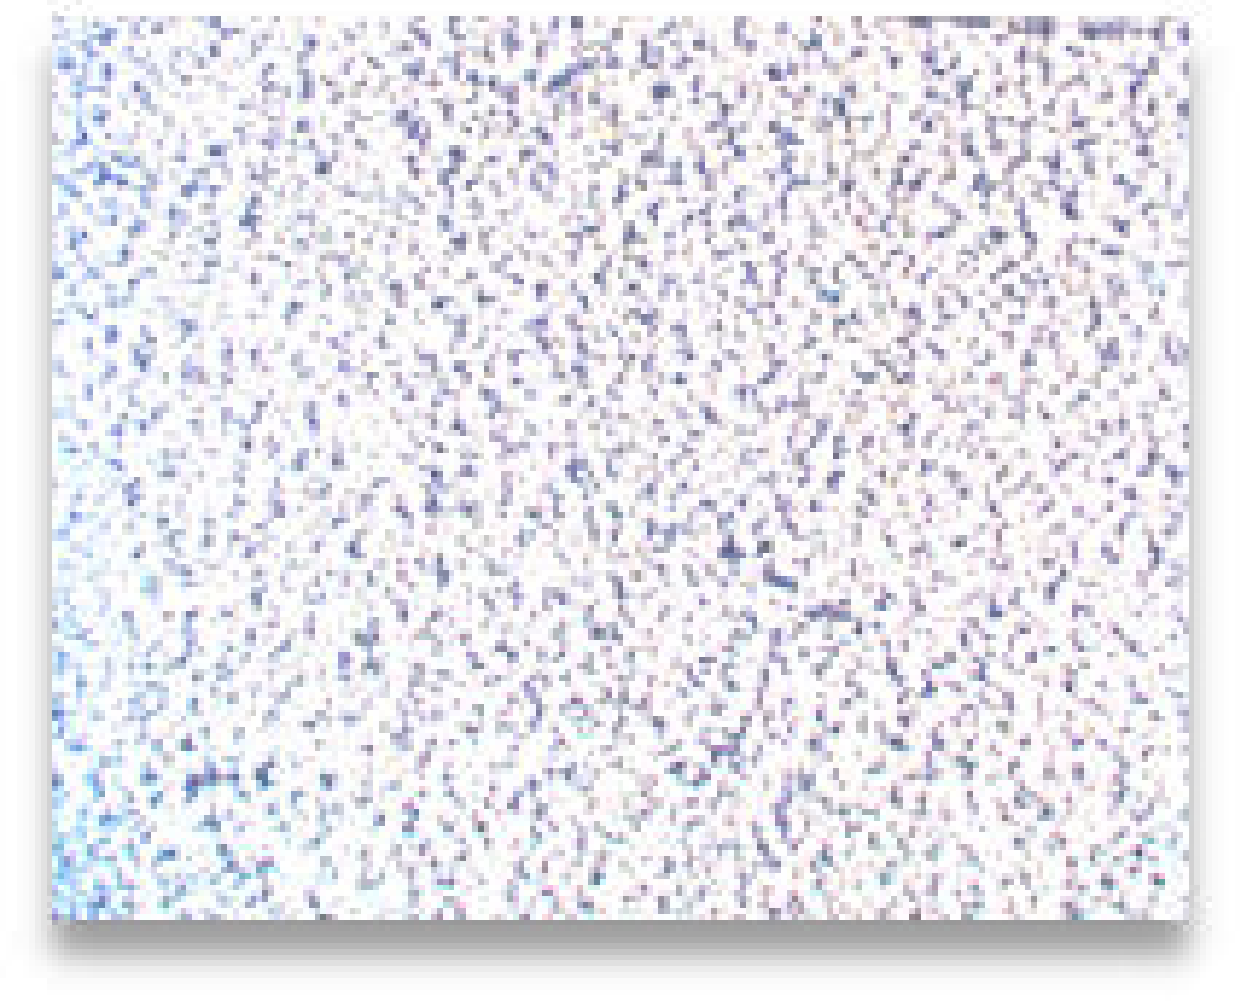
\includegraphics[width=4cm]{./Ch3_SoilTypeDiscrimination/Fig/C_K1_image_compressed.pdf}
			\caption*{(c)土の種類C(粗粒土)} % 硅砂1号
			\end{minipage}

			\\

			\begin{minipage}[t]{0.33\linewidth}
			
\includegraphics[width=4cm]{./Ch3_SoilTypeDiscrimination/Fig/D_K9_image_compressed.pdf}
			\caption*{(d)土の種類D(粘性土)} % 硅砂9号
			% \vspace{2cm}
			\end{minipage}

			\begin{minipage}[t]{0.33\linewidth}
			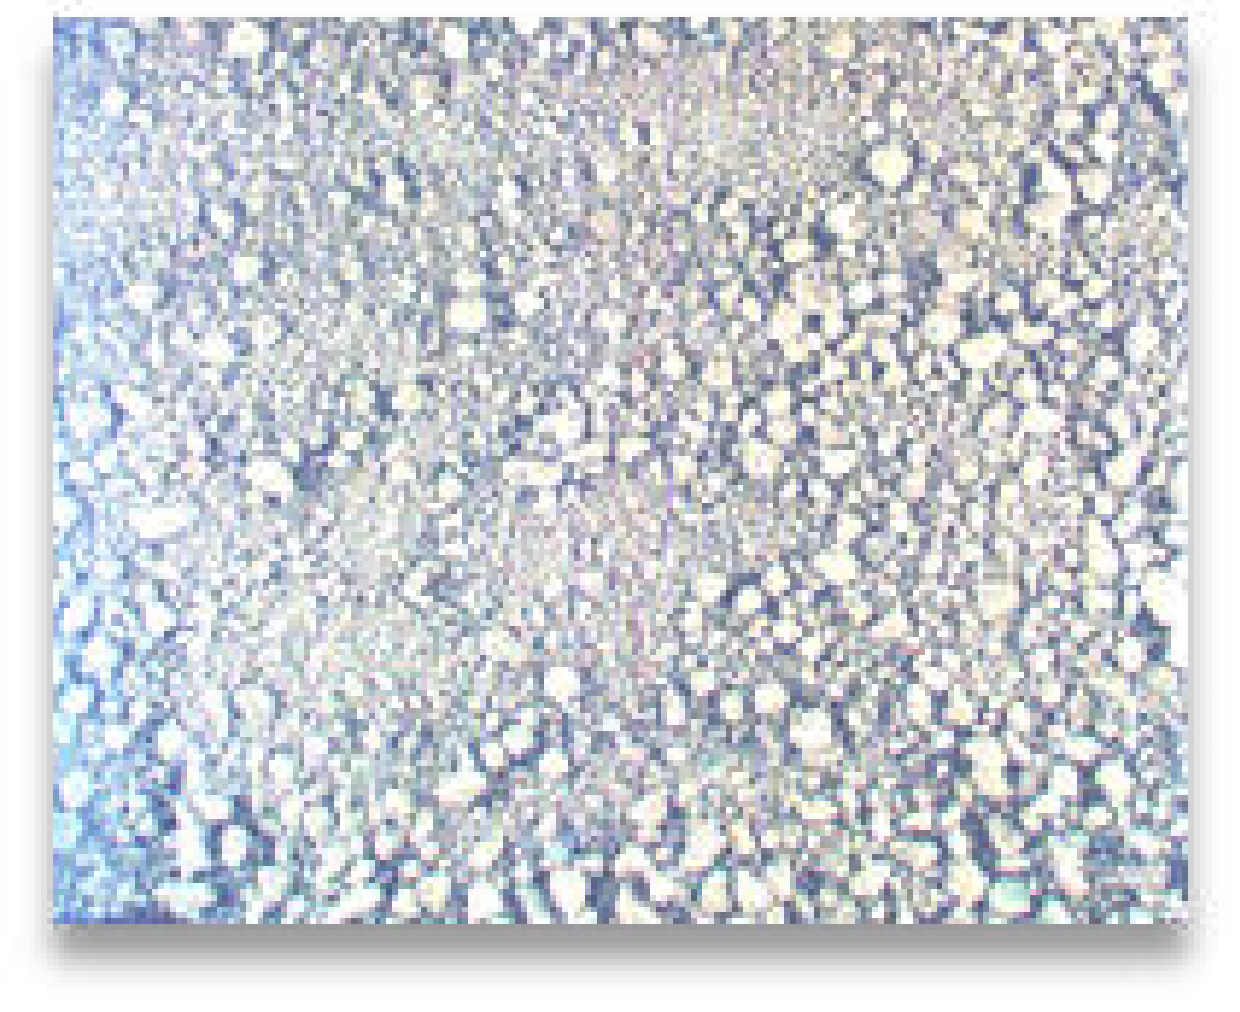
\includegraphics[width=4cm]{./Ch3_SoilTypeDiscrimination/Fig/E_Ko_image_compressed.pdf}
			\caption*{(e)土の種類E(粗粒土)} % 三重県三重郡
			\end{minipage}

			\hfill

			\begin{minipage}[t]{0.33\linewidth}
			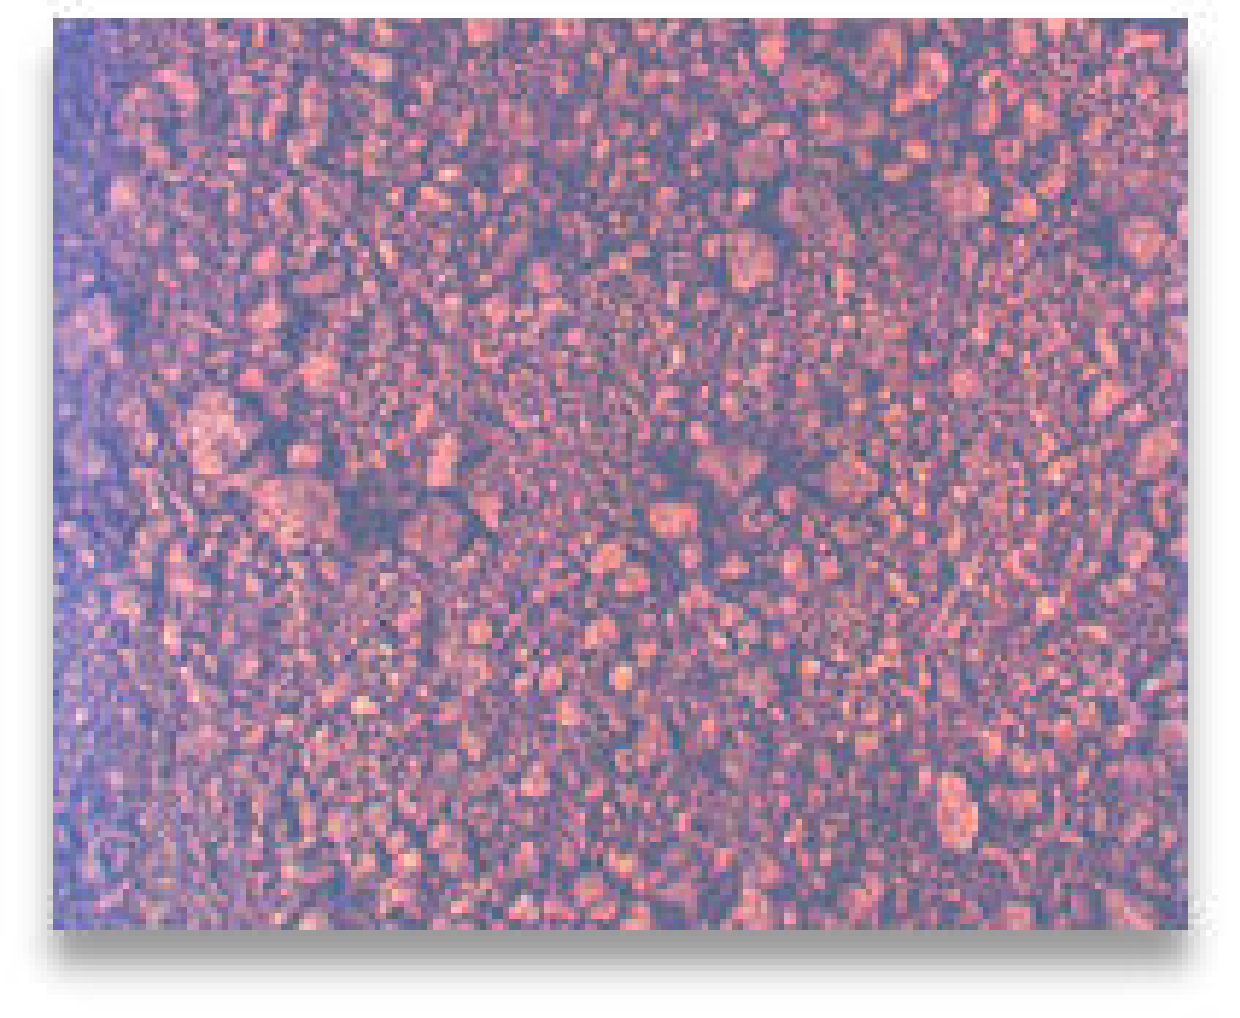
\includegraphics[width=4cm]{./Ch3_SoilTypeDiscrimination/Fig/F_Lo_image_compressed.pdf}
			\caption*{(f)土の種類F(火山灰質粘性土)} % 静岡県御殿場市
			\end{minipage}

			\\

			\begin{minipage}[t]{0.33\linewidth}
			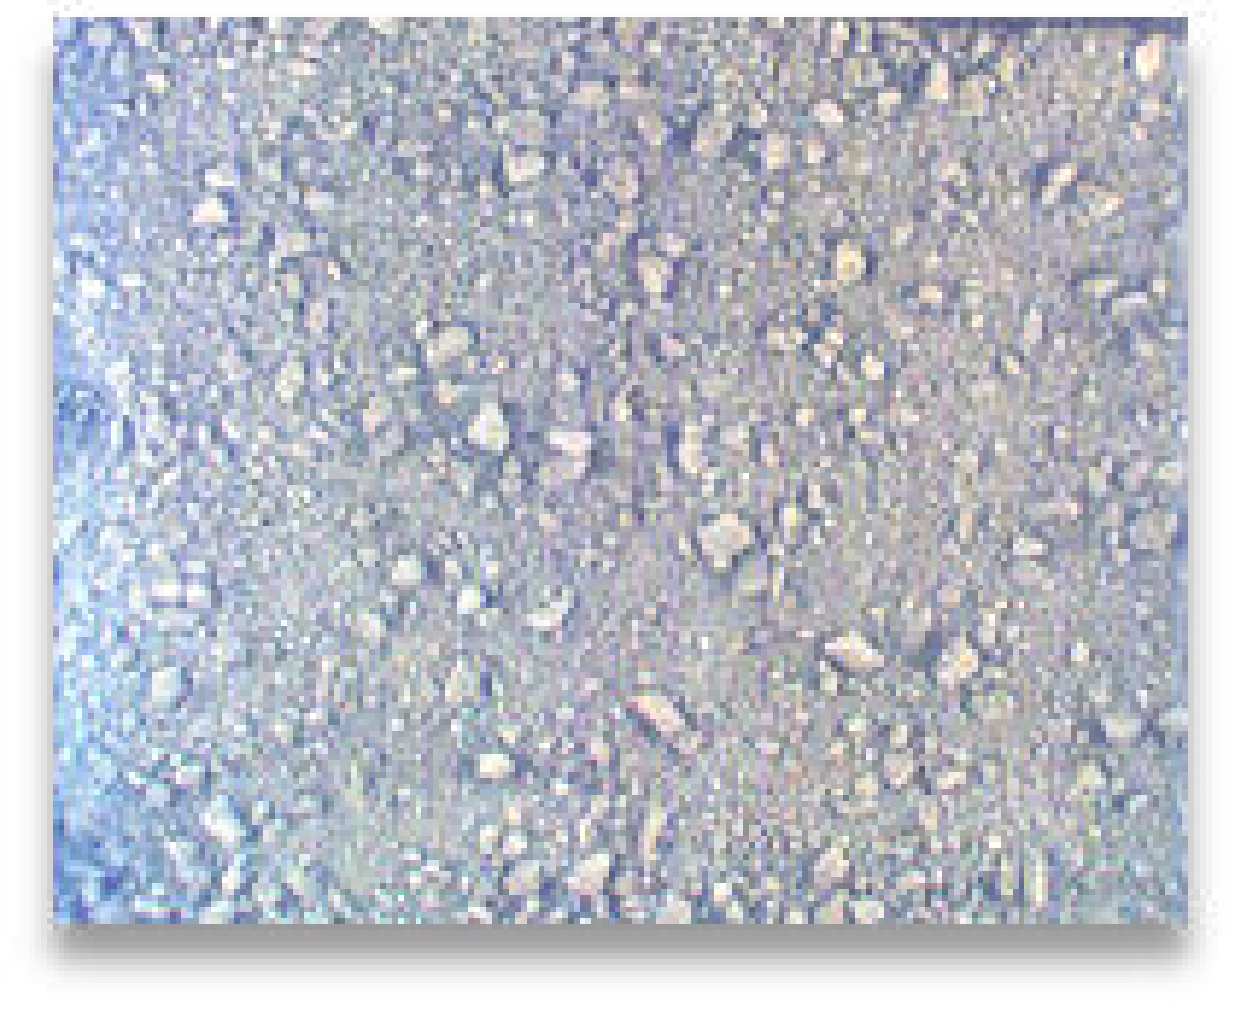
\includegraphics[width=4cm]{./Ch3_SoilTypeDiscrimination/Fig/G_Mi_image_compressed.pdf}
			\caption*{(g)土の種類G(粘性土)} % 宮崎県?
 			% \vspace{2cm}
			\end{minipage}

			\begin{minipage}[t]{0.33\linewidth}
			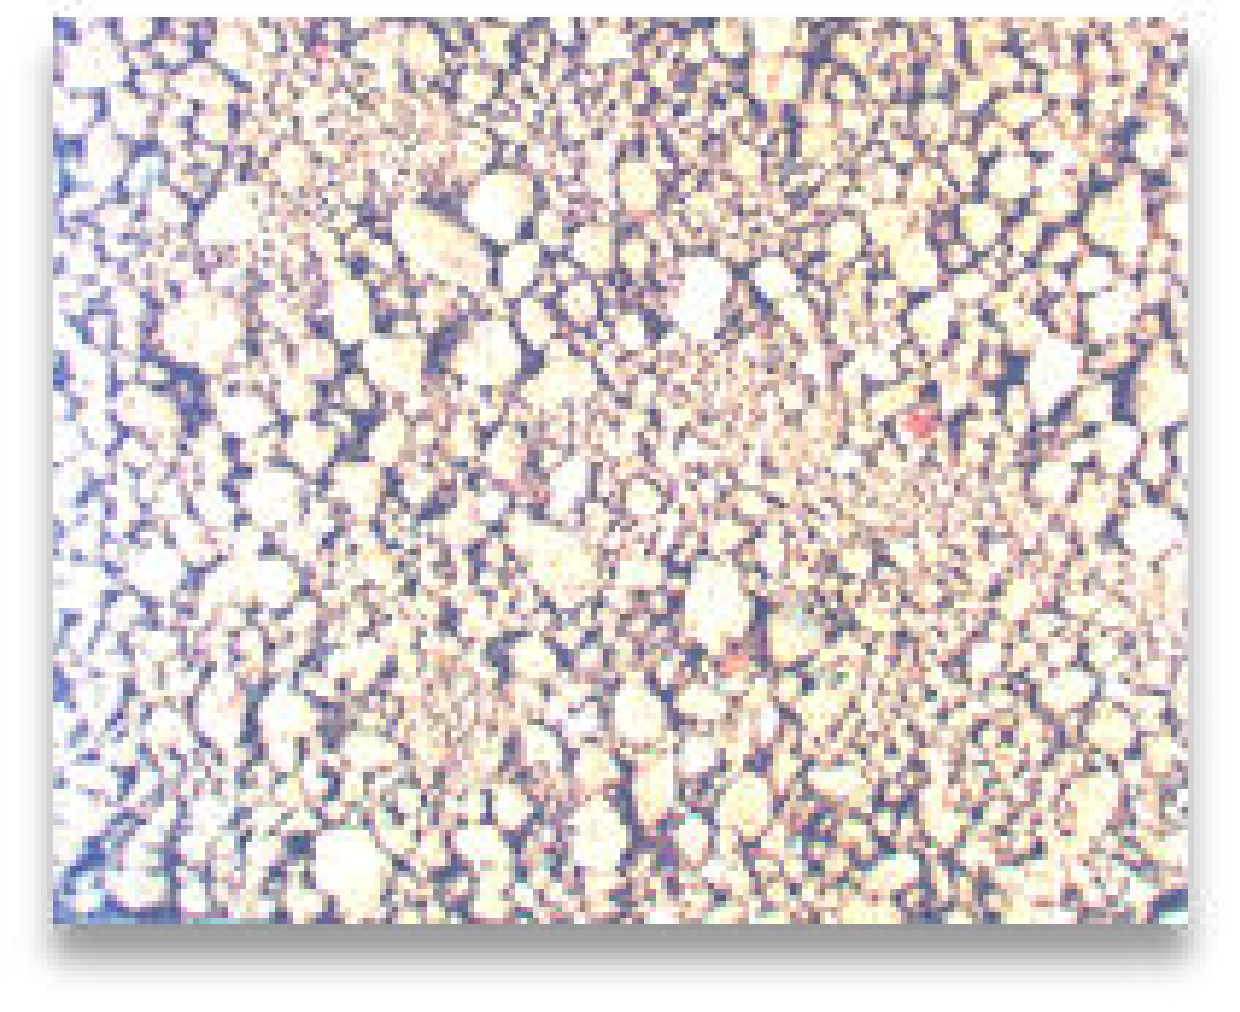
\includegraphics[width=4cm]{./Ch3_SoilTypeDiscrimination/Fig/H_Oh_image_compressed.pdf}
			\caption*{(h)土の種類H(粗粒土)} % 北海道?,青森県?,岩手県?
			\end{minipage}

			\hfill

			\begin{minipage}[t]{0.33\linewidth}
			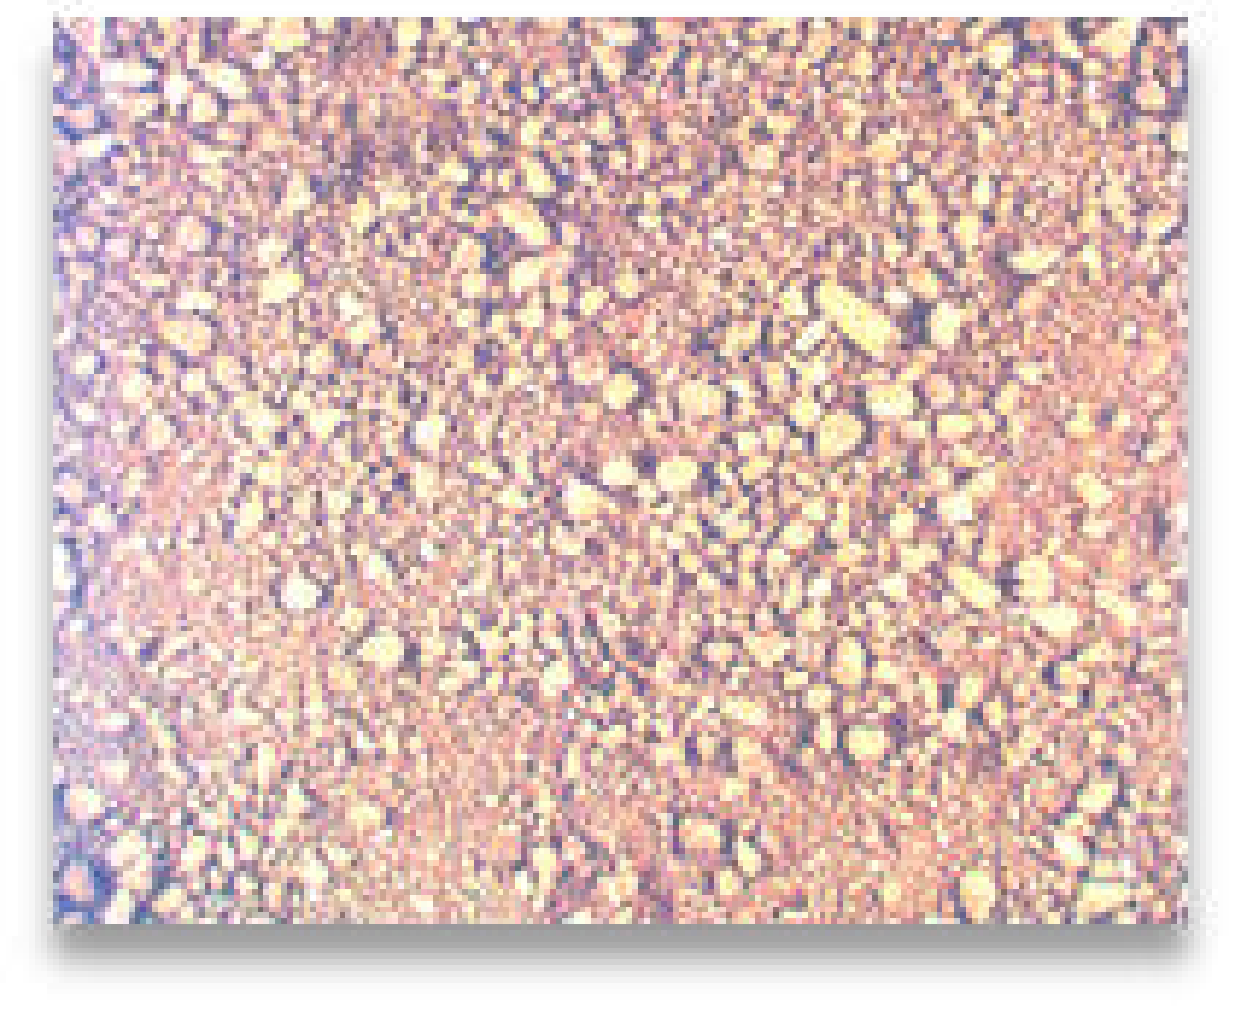
\includegraphics[width=4cm]{./Ch3_SoilTypeDiscrimination/Fig/I_Sa_image_compressed.pdf}
			\caption*{(i)土の種類I(粗粒土)} % 大阪府茨木市
			\end{minipage}

			\\

			\begin{minipage}[t]{0.33\linewidth}
			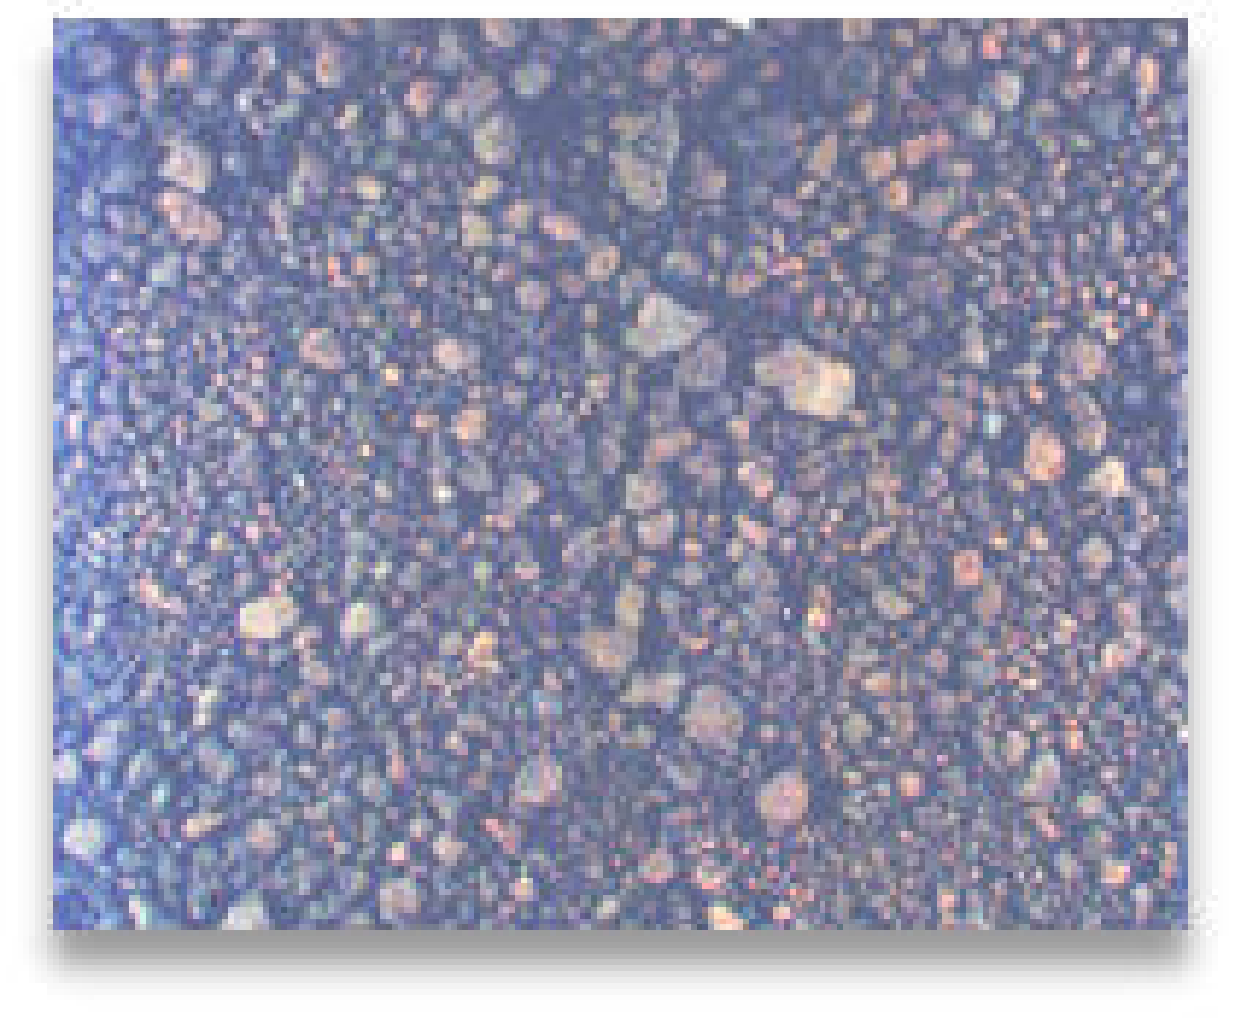
\includegraphics[width=4cm]{./Ch3_SoilTypeDiscrimination/Fig/J_Sc_image_compressed.pdf}
			\caption*{(j)土の種類J(粗粒土)} % 静岡県御殿場市
			\end{minipage}

		\end{tabular}
		\caption{土の種類を識別する検証実験用のデータ}\label{fig:discrimination_experiment_data}
	\end{center}
\end{figure}

\clearpage

\subsection{実験結果}
\label{ssec:DiscriminationResult}

\ref{ssec:NeuralNetWork}項で解説したニューラルネットワークを,
バッチサイズを128,エポック数を12に設定して学習を行った.
学習したニューラルネットワークを用いて,10種類の土を撮影したマルチスペクトル画像から取得した
分光反射率スペクトルを識別した結果の混同行列を
図\ref{fig:discrimination_confusion_matrix}に示す.
% このニューラルネットワークのトレーニングは,.
この混同行列は,縦軸がマルチスペクトル画像の各画素の分光反射率スペクトルの実際の土の種類を示し,
横軸がその分光反射率スペクトルをニューラルネットワークで識別した結果を示す.
各分光反射率スペクトルが撮影された実際の土の種類と,ニューラルネットワークによって識別された土の種類が一致した
場合は,混同行列の対角成分の部分の確率が高くなる.
この混同行列における確率は,高くなるほど濃い青色になる.
確率と色の濃さの対応を,図\ref{fig:discrimination_confusion_matrix}の右側にあるカラーバーに示す.
この混同行列から分かる通り,使用した10種類の土全てにおいて高い確率で
分光反射率スペクトルから実際の土の種類を識別できていることが分かる.
また,今回のニューラルネットワークによる土の種類の識別の結果,
全体の正解率が81.57\%となった.

\begin{figure}[b]
	\begin{center}
	\centering
	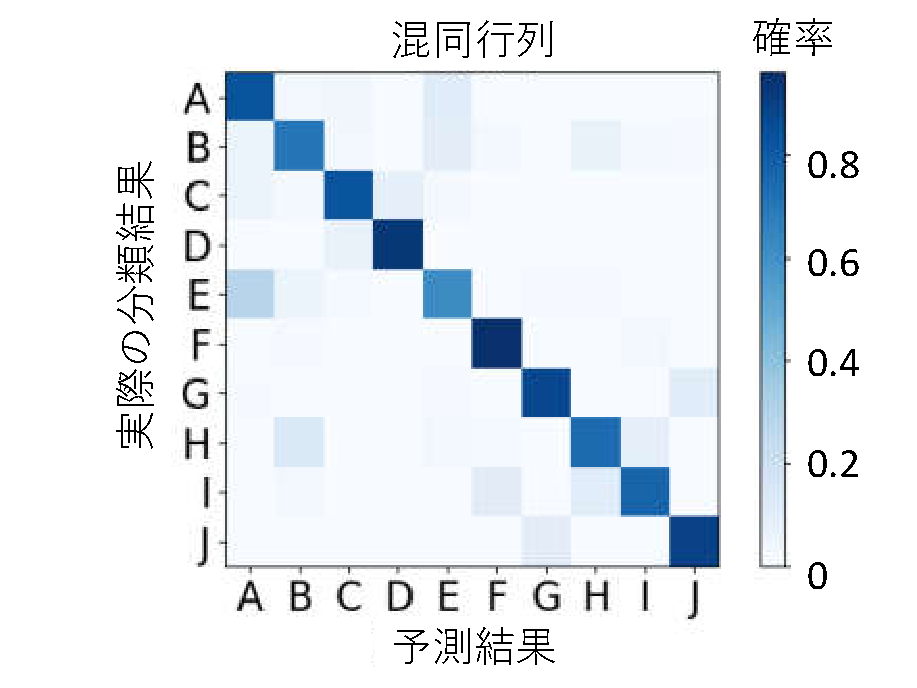
\includegraphics[width=8cm]{./Ch3_SoilTypeDiscrimination/Fig/confusion_matrix_compressed.pdf}
	\caption{10種類の土の識別結果を示す混同行列}\label{fig:discrimination_confusion_matrix}
	\end{center}
\end{figure}

\clearpage

\subsection{考察}
\label{ssec:DiscriminationConsideration}

今回の検証実験の結果より,マルチスペクトル画像から取得した分光反射率スペクトルを用いた土の種類の識別精度は
高いことが分かった.
従って,土の種類の違いによる分光反射率スペクトルの違いから,ニューラルネットワークを用いることによって
高い精度で土の種類を識別できることが確認出来た.
これは,マルチスペクトル画像から幅の狭い波長帯を数多く取得することによって
非常に多くの波長帯の光の強さを記録する分光反射率スペクトルを取得し,
1つの土の種類に対して十分詳細な分光反射率スペクトルの形状をニューラルネットワークに学習させることが
できたためである.
また,この\ref{sec:PreliminaryExperimentOfDiscrimination}節で解説した土の種類を識別する検証実験では,
マルチスペクトル画像を屋内の暗室でハロゲンランプを光源にして撮影したが,
\ref{ssec:DiscriminationExperimentSetting}項で述べた通り,
ハロゲンランプと太陽光は似たスペクトルを持つため,太陽光を光源にしても,
土の種類の違いによる分光反射率スペクトルの違いをニューラルネットワークによって捉え,
高精度で土の種類を識別することが期待できる.

% "詳細"と"詳細でない"の違いを明確にして

% 非常に多くの波長帯の光の強さを記録する
% % 波長分解能の高い why
% 分光反射率スペクトル

しかし,一部の土では少し推定精度が落ちることも分かった.
例えば,図\ref{fig:discrimination_confusion_matrix}の混同行列における各成分の確率より,
実際の種類はEである土がAであると識別されたり,実際の種類はHである土がBやIと識別される確率が
僅かに他の誤認識の場合に比べて高いことが分かる.
図\ref{fig:discrimination_experiment_data}において,
土の種類Eと土の種類A,あるいは土の種類H,土の種類B,および土の種類IのRGB画像を比較すると,
それぞれ土粒子の大きさが多少異なっているが,
EとAは共に白みががっており,H,B,およびIは共に赤みががっていることが分かる.
よって,似た色あいの土の種類は分光反射率スペクトルが似た形状になるため,
識別精度が落ちることが分かる.
本研究では,分光反射率スペクトルを用いて土の種類を識別するため,
土の粒子の材質に比べて粒度分布の情報を取得しにくいと考えられる.
このような誤認識を低減させるためには,
マルチスペクトル画像の画素ごとの分光反射率スペクトルのみを考慮するのではなく,
マルチスペクトル画像のテクスチャも考慮する必要がある.

\newpage


%==============================================================================
%おわりに
%==============================================================================
\section{おわりに}

本章では,非接触での走破性判定のために本研究で提案した,スペクトル画像を用いたコーン指数推定の最初のステップである,
マルチスペクトル画像から取得した分光反射率スペクトルを用いた土の種類の識別の詳細について述べた.

まず,\ref{sec:SoilTypeDiscriminationFromSpectrum}節において,
土の種類が異なると分光反射率スペクトルも異なることを利用して,分光反射率スペクトルを用いて
土の種類を識別することを述べた.
更に,分光反射率スペクトルから多数の土の種類を識別するためには,
波長分解能の高い分光反射率スペクトルを使用する必要がある.
そのためには,入射光を幅の短い多数の波長帯に分光させて,
非常に多くの波長帯の光の強さを記録する必要がある.
% 多くの波長帯に分光させて記録した
% 詳細な形状の分光反射率スペクトルを知る必要がある.
そのために,マルチスペクトル画像の中でも,分光させる波長の数が非常に多い
マルチスペクトル画像を使用することも述べた.

次に,\ref{sec:ClassificationOfHyperspectralImage}節において,
本研究で使用するマルチスペクトル画像には1画素ごとにその画素に写りこんだ
物質の分光反射率スペクトルが記録されているため,
それを1画素ごと取得してニューラルネットワークを用いることで土の種類を識別することを述べた.

最後に,\ref{sec:PreliminaryExperimentOfDiscrimination}節において,
\ref{sec:SoilTypeDiscriminationFromSpectrum}節と\ref{sec:ClassificationOfHyperspectralImage}で
解説した,マルチスペクトル画像から取得した分光反射率スペクトルを用いた土の種類の識別が実際に可能か確認するための
検証実験の詳細について述べた.
この検証実験では,暗室において,ハロゲンランプを光源として撮影したマルチスペクトル画像から分光反射率スペクトルを取得した.
そして,10種類の土を集めて,識別が可能か確認した.
検証実験の結果より,土の種類の違いによって変動する分光反射率スペクトルの違いを,
ニューラルネットワークを用いて高い精度で識別できることが分かった.

\newpage
%%%%%%%%%%%%%%%%%%%%%%%%%%%%%%%%%%%%%%%%%%%%%%%%%%%%%%%%%%%%%%%%%%%%%%%%%%%%%%%